% Options for packages loaded elsewhere
\PassOptionsToPackage{unicode}{hyperref}
\PassOptionsToPackage{hyphens}{url}
\documentclass[
  10pt,
]{article}
\usepackage{xcolor}
\usepackage[margin=0.8in]{geometry}
\usepackage{amsmath,amssymb}
\setcounter{secnumdepth}{-\maxdimen} % remove section numbering
\usepackage{iftex}
\ifPDFTeX
  \usepackage[T1]{fontenc}
  \usepackage[utf8]{inputenc}
  \usepackage{textcomp} % provide euro and other symbols
\else % if luatex or xetex
  \usepackage{unicode-math} % this also loads fontspec
  \defaultfontfeatures{Scale=MatchLowercase}
  \defaultfontfeatures[\rmfamily]{Ligatures=TeX,Scale=1}
\fi
\usepackage{lmodern}
\ifPDFTeX\else
  % xetex/luatex font selection
\fi
% Use upquote if available, for straight quotes in verbatim environments
\IfFileExists{upquote.sty}{\usepackage{upquote}}{}
\IfFileExists{microtype.sty}{% use microtype if available
  \usepackage[]{microtype}
  \UseMicrotypeSet[protrusion]{basicmath} % disable protrusion for tt fonts
}{}
\makeatletter
\@ifundefined{KOMAClassName}{% if non-KOMA class
  \IfFileExists{parskip.sty}{%
    \usepackage{parskip}
  }{% else
    \setlength{\parindent}{0pt}
    \setlength{\parskip}{6pt plus 2pt minus 1pt}}
}{% if KOMA class
  \KOMAoptions{parskip=half}}
\makeatother
\usepackage{longtable,booktabs,array}
\newcounter{none} % for unnumbered tables
\usepackage{calc} % for calculating minipage widths
% Correct order of tables after \paragraph or \subparagraph
\usepackage{etoolbox}
\makeatletter
\patchcmd\longtable{\par}{\if@noskipsec\mbox{}\fi\par}{}{}
\makeatother
% Allow footnotes in longtable head/foot
\IfFileExists{footnotehyper.sty}{\usepackage{footnotehyper}}{\usepackage{footnote}}
\makesavenoteenv{longtable}
\usepackage{graphicx}
\makeatletter
\newsavebox\pandoc@box
\newcommand*\pandocbounded[1]{% scales image to fit in text height/width
  \sbox\pandoc@box{#1}%
  \Gscale@div\@tempa{\textheight}{\dimexpr\ht\pandoc@box+\dp\pandoc@box\relax}%
  \Gscale@div\@tempb{\linewidth}{\wd\pandoc@box}%
  \ifdim\@tempb\p@<\@tempa\p@\let\@tempa\@tempb\fi% select the smaller of both
  \ifdim\@tempa\p@<\p@\scalebox{\@tempa}{\usebox\pandoc@box}%
  \else\usebox{\pandoc@box}%
  \fi%
}
% Set default figure placement to htbp
\def\fps@figure{htbp}
\makeatother
\setlength{\emergencystretch}{3em} % prevent overfull lines
\providecommand{\tightlist}{%
  \setlength{\itemsep}{0pt}\setlength{\parskip}{0pt}}
\usepackage{float}
\floatplacement{figure}{H}
\usepackage{bookmark}
\IfFileExists{xurl.sty}{\usepackage{xurl}}{} % add URL line breaks if available
\urlstyle{same}
\hypersetup{
  pdftitle={The Spatial Distribution of Farmers Markets in Philadelphia},
  hidelinks,
  pdfcreator={LaTeX via pandoc}}

\title{The Spatial Distribution of Farmers Markets in Philadelphia}
\usepackage{etoolbox}
\makeatletter
\providecommand{\subtitle}[1]{% add subtitle to \maketitle
  \apptocmd{\@title}{\par {\large #1 \par}}{}{}
}
\makeatother
\subtitle{Homework 4 \textbar{} CPLN 671 / MUSA 500}
\author{}
\date{\vspace{-2.5em}November 28, 2026}

\begin{document}
\maketitle

\section{A. Introduction}\label{a.-introduction}

Farmers markets can improve access to fresh food, but their benefits
depend partly on where they operate. This report examines whether
Philadelphia's 2013 farmers markets were randomly distributed,
clustered, or dispersed within the city. It uses nearest neighbor
analysis and Ripley's K-function to examine different spatial scales,
then compares market locations with ZIP-code median household income.
These analyses describe geographic patterns; they do not directly
measure residents' travel access or explain why markets chose particular
locations.

\section{B. Methods}\label{b.-methods}

\subsection{B.a. Complete spatial randomness and
hypotheses}\label{b.a.-complete-spatial-randomness-and-hypotheses}

Complete spatial randomness (CSR) means a homogeneous Poisson process:
intensity is constant across the study area, and counts in disjoint
areas are independent. Conditional on the observed number of markets,
locations are independent and uniformly distributed within Philadelphia.
The null hypothesis is CSR. Alternatives are clustering, with more
nearby points than CSR predicts, or dispersion, with fewer nearby
points. Statistical departures are assessed at the 5\% level, with the
specific simulation-envelope level explained below. Rejecting CSR alone
does not distinguish interactions between markets from differences in
population or suitable land.

\subsection{B.b. Quadrat analysis}\label{b.b.-quadrat-analysis}

Quadrat analysis divides the study area into cells and compares their
point counts with counts expected under CSR. Equal-area cells have equal
expected counts; boundary cells require adjustments for their smaller
areas. A variance substantially above the mean suggests clustering,
whereas a smaller variance suggests regularity. A count-based
goodness-of-fit test can assess departures from the null. However,
results depend strongly on grid size, shape, and placement; sparse cells
undermine approximations, and counts discard locations within cells.
These limitations make quadrats a less informative stand-alone method
here. Quadrat analysis was not performed.

\subsection{B.c. Nearest neighbor
analysis}\label{b.c.-nearest-neighbor-analysis}

The study window is the supplied Philadelphia boundary, covering
approximately 142.4 square miles. All 62 market records are retained,
including two separately listed businesses at the Reading Terminal
location. Coordinates use Pennsylvania South State Plane, EPSG:2272, in
US survey feet. Nearest neighbor analysis averages the straight-line
distance from each market to its closest other market. With \(n\)
points, area \(A\), intensity \(\lambda=n/A\), and nearest neighbor
distances \(d_i\),

\[
\bar d_o=\frac{1}{n}\sum_{i=1}^{n}d_i,\qquad
\bar d_e=\frac{1}{2\sqrt{\lambda}},\qquad
R=\frac{\bar d_o}{\bar d_e}.
\]

The conventional approximate CSR test uses

\[
SE=\sqrt{\frac{4-\pi}{4\pi\lambda n}},\qquad
z=\frac{\bar d_o-\bar d_e}{SE}.
\]

Here \(\bar d_o\) and \(\bar d_e\) are the observed and expected means,
and \(SE\) is the standard error. Values \(R<1\) suggest clustering;
\(R>1\) suggests dispersion. A two-sided test rejects when \(|z|>1.96\)
at \(\alpha=0.05\). The R analysis also checks the conclusion using the
boundary-adjusted Clark-Evans test and 99 uniform simulations in the
same window.

This method summarizes only the closest neighbor, depends on the chosen
boundary, and can miss patterns at larger scales. A hospital analogy
illustrates another limitation: facilities can be close together because
they serve concentrated populations, without attracting one another.
Markets likewise depend on customers and available sites. Straight-line
distances also omit street routes and travel barriers.

\subsection{B.d.i--ii. K/L functions and distance
settings}\label{b.d.iii.-kl-functions-and-distance-settings}

K-function analysis counts all other points within distance \(d\) of a
typical point, scaled by intensity:

\[
K(d)=\frac{E[\text{number of other points within }d]}{\lambda},
\qquad K_{CSR}(d)=\pi d^2.
\]

The R function \texttt{Kest} estimates

\[
\widehat K(d)=\frac{A}{n(n-1)}
\sum_i\sum_{j\ne i}I(d_{ij}\le d)e_{ij},
\]

where \(d_{ij}\) is pairwise distance, \(I\) indicates whether the pair
is within \(d\), and \(e_{ij}\) is its edge weight.
\href{https://search.r-project.org/CRAN/refmans/spatstat.explore/html/Kest.html}{Kest
documentation}

The usual transformation is \(L(d)=\sqrt{K(d)/\pi}\), whose CSR
benchmark is \(d\). Our script plots the centered form
\(L_c(d)=L(d)-d\), although the saved figure calls it ``L.'' Its CSR
benchmark is zero. Positive values indicate an excess of nearby pairs
relative to homogeneous CSR; they are not literal extra neighbors or
additional travel distances.
\href{https://search.r-project.org/CRAN/refmans/spatstat.explore/html/Lest.html}{L-function
documentation}

Following the assignment, the script begins at zero and uses ten
increments of 2,500 feet: \(d_j=0+2,500j\), \(j=1,\ldots,10\). Thus
reported positive distances span 2,500--25,000 feet. These are
prescribed settings rather than estimated travel thresholds; a 100-foot
grid draws the curves between reported distances.

\subsection{B.d.iii. Simulation
envelopes}\label{b.d.iii.-simulation-envelopes}

The analysis generates 99 independent uniform patterns, each containing
62 points inside the same city boundary, using seed 671. Each receives
the same K estimator. The minimum and maximum simulated values at each
distance form a pointwise envelope. An observed curve above it supports
clustering at that distance; below it supports dispersion. For a fixed
distance, the min/max envelope has nominal two-sided rejection level
\(2/(99+1)=0.02\), subject to ties. It is not a simultaneous 95\%
confidence band. The one-sided clustering probability is

\[
p(d)=\frac{1+\#\{\widehat K_{sim}(d)\ge\widehat K_{obs}(d)\}}{100}.
\]

Its minimum is 0.01. Examining many distances does not turn these
pointwise comparisons into one global test.
\href{https://search.r-project.org/CRAN/refmans/spatstat.explore/help/envelope.html}{Envelope
documentation}

\subsection{B.d.iv. Boundary
correction}\label{b.d.iv.-boundary-correction}

Markets near a boundary may have unobserved neighbors outside the
window, causing undercounts. Ripley's isotropic correction increases a
pair's contribution according to the fraction of its circular
neighborhood that is observable. The R analysis uses this correction
because \texttt{Kest} supports Philadelphia's polygonal window. ArcGIS's
Simulate Outer Boundary Values method instead adds mirrored points
outside the boundary for neighbor counting. It is distinct from
generating the 99 reference patterns. The assignment requests that
ArcGIS method; the supplied R results are a substitute and do not
reproduce that setting.
\href{https://pro.arcgis.com/en/pro-app/3.4/tool-reference/spatial-statistics/multi-distance-spatial-cluster-analysis.htm}{Esri
documentation}

\subsection{B.d.v. Population-based inhomogeneous K (Part
C)}\label{b.d.v.-population-based-inhomogeneous-k-part-c}

Uniform CSR may be inappropriate if markets follow an unevenly
distributed population. We construct an external reference from the
supplied \textbf{2000 ZIP populations}, rather than estimate intensity
from the market locations themselves. Each ZIP's population is divided
by its polygon area, assigned to a 250-foot grid, and Gaussian-smoothed
with a one-mile (5,280-foot) standard deviation. Boundary normalization
prevents artificially low values at the city edge. The resulting surface
is rescaled so its integral over Philadelphia equals 62 expected
markets. Grid size and smoothing distance are modeling choices, not
observed service areas. ZIP 19112's recorded zero population is retained
before smoothing; nearby population supplies positive smoothed
intensity. No area is removed from the city window.

\texttt{Kinhom} weights each pair by the inverse of its two local
intensities and applies isotropic edge correction. We set
\texttt{renormalise=FALSE} because the population-based surface has
already been scaled, and use the same 0--25,000-foot radius grid as Part
B. We report \(L_{inhom,c}(d)=\sqrt{K_{inhom}(d)/\pi}-d\); the Poisson
reference is zero. Ninety-nine independent inhomogeneous Poisson
patterns are simulated inside the \textbf{original city polygon} using
seed 671. Their expected count is 62, but their realized counts vary.
Each simulated curve receives the same estimator and fixed intensity
surface.

The min/max envelope is pointwise and exploratory: intensity's total
rate is fitted from the observed count, and uncertainty about
population, smoothing, and the historical data is not simulated. Unlike
Part B's fixed-count simulations, these allow count variation; therefore
a wider envelope cannot be attributed to population adjustment alone. A
curve inside this envelope is compatible with this particular reference,
not proof that population fully explains market placement.

\newpage

\section{C. Results}\label{c.-results}

\subsection{C.a. Nearest neighbor
analysis}\label{c.a.-nearest-neighbor-analysis}

Mean nearest neighbor distance is 3,112.9 feet, compared with a CSR
expectation of 4,001.4 feet. The index is \(R=0.778\), with \(z=-3.345\)
and two-sided \(p=0.000824\). We reject CSR in the direction of
clustering. The boundary-adjusted Clark--Evans result (\(R=0.7091\);
two-sided \(p=0.00001176\)) and the simulation check (one-sided
\(p=0.01\)) support this conclusion.

\subsection{C.b.i. K-function
analysis}\label{c.b.i.-k-function-analysis}

Using the prescribed zero beginning distance and 2,500-foot increments,
observed K exceeds the simulation envelope at all ten positive reported
distances, 2,500--25,000 feet. Each has a one-sided rank \(p=0.01\),
supporting rejection of homogeneous CSR toward clustering at those
distances. At 2,500 feet, observed K is 37.8 million square feet, above
the upper envelope of 31.8 million. At 25,000 feet, it is 3.11 billion,
above 2.26 billion. These are cumulative neighborhoods, not ten separate
rings.

Centered L is positive at every reported distance and reaches 7,260 feet
at the 20,000-foot band. This summarizes the transformed departure from
CSR, not a literal gain in distance or neighbors. The 22,500- and
25,000-foot bands exceed the approximately 22,384-foot recommended range
recorded in the analysis, so the largest-distance estimates merit
caution. These pointwise results agree with nearest neighbor analysis
without establishing a global envelope test or a population-adjusted
conclusion.

\begin{figure}
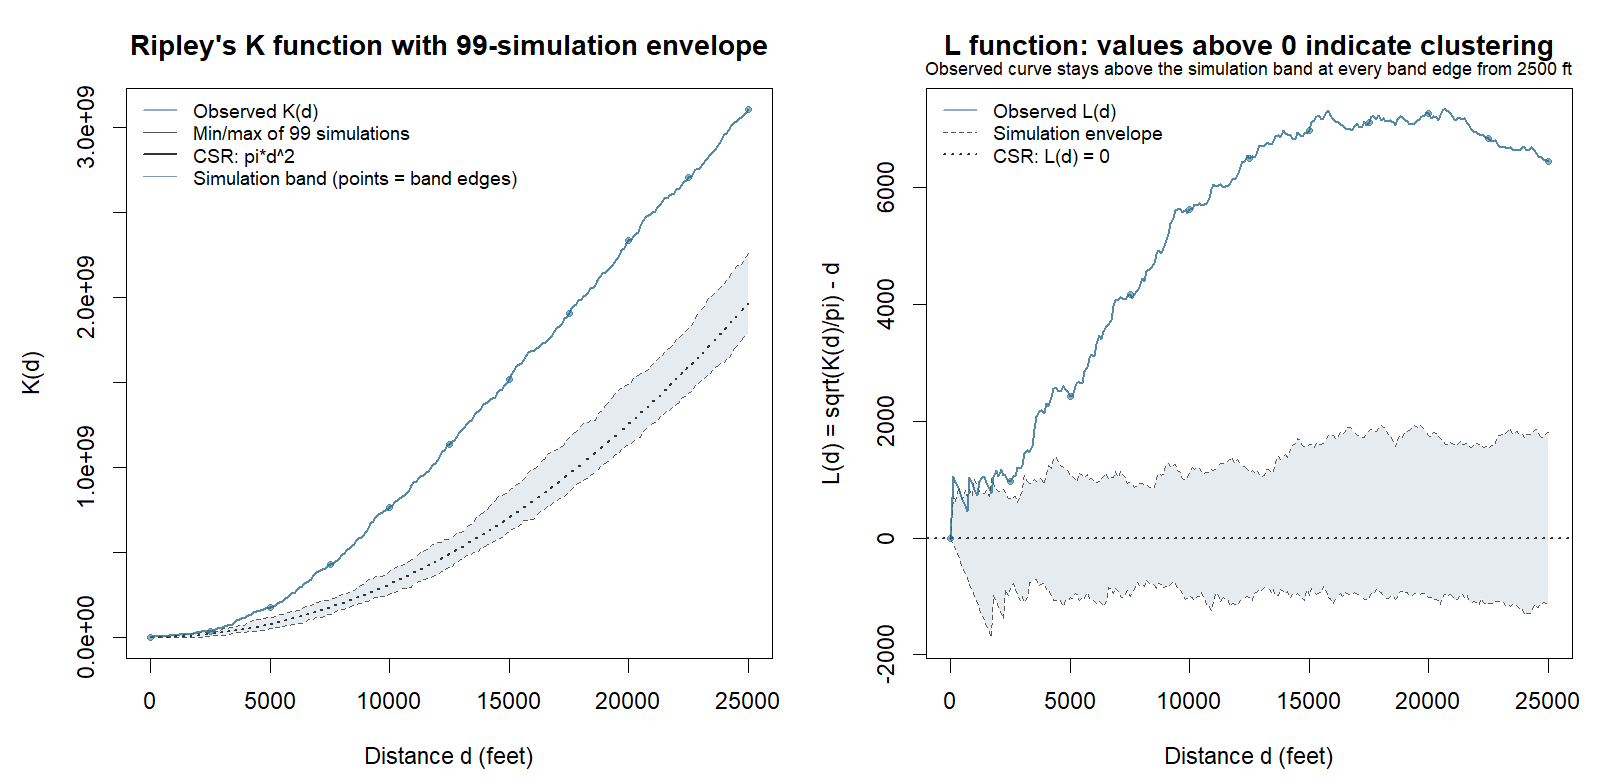
\includegraphics[width=1\linewidth]{../output/fig_04_kfunction_envelope} \caption{Part B: homogeneous K and centered L with the min/max envelope of 99 fixed-count CSR simulations. These are pointwise comparisons.}\label{fig:k-curve}
\end{figure}

\newpage

\subsection{C.b.ii. Population reference and geographic gaps (Part
C)}\label{c.b.ii.-population-reference-and-geographic-gaps-part-c}

Low population alone is not a convincing explanation for the
northeastern gap. For example, ZIPs 19111 and 19149 contain 58,672 and
48,857 residents in the supplied 2000 data but no market records in
2013. Seven selected northeastern ZIPs (19111, 19114, 19115, 19116,
19149, 19152, and 19154) together contain \textbf{270,209 residents} and
zero listed markets. This describes those ZIPs, not a formally defined
regional boundary or residents' ability to cross a ZIP boundary to shop.

The assignment asks for an expectation without running an additional
analysis: we would expect population adjustment to reduce some apparent
citywide clustering, while populated areas without markets would remain
policy-relevant. As an additional Part C analysis, the observed Kinhom
curve is \textbf{inside the simulated envelope at all ten positive
reported distances}. Its smallest one-sided clustering rank probability
is 0.10. Thus this exploratory analysis does not detect excess
clustering beyond the chosen population-based reference at these band
edges.

For context, at 10,000 feet centered L decreases from 5,619 feet in Part
B to 1,879 feet in Part C. This suggests that allowing uneven intensity
changes the interpretation substantially. It does \textbf{not} establish
that population is the sole explanation, particularly given the
differing count assumptions and broad reference envelope.

\begin{figure}
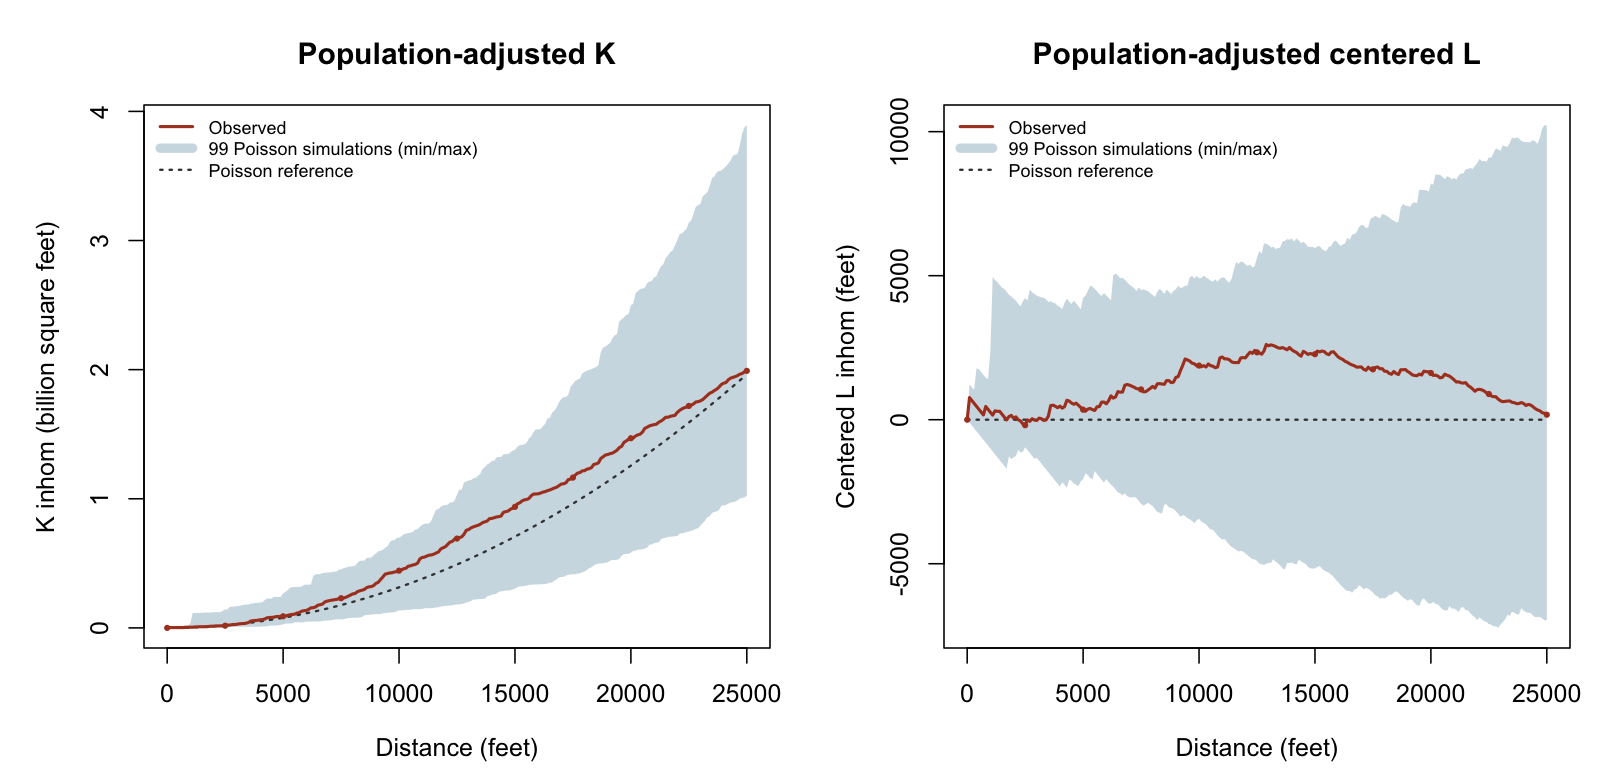
\includegraphics[width=0.9\linewidth]{../output/fig_08_kinhom_curves} \caption{Population-based Kinhom and centered L. Shading is the min/max of 99 plug-in Poisson simulations, not a simultaneous confidence band.}\label{fig:adjusted-curve}
\end{figure}

\begin{longtable}[]{@{}rrrl@{}}
\caption{Population-adjusted results at the ten prescribed band
edges.}\tabularnewline
\toprule\noalign{}
Distance (ft) & Centered L (ft) & Upper-tail rank p & Envelope
position \\
\midrule\noalign{}
\endfirsthead
\toprule\noalign{}
Distance (ft) & Centered L (ft) & Upper-tail rank p & Envelope
position \\
\midrule\noalign{}
\endhead
\bottomrule\noalign{}
\endlastfoot
2500 & -191 & 0.48 & inside \\
5000 & 348 & 0.33 & inside \\
7500 & 1052 & 0.14 & inside \\
10000 & 1879 & 0.10 & inside \\
12500 & 2339 & 0.12 & inside \\
15000 & 2274 & 0.11 & inside \\
17500 & 1748 & 0.20 & inside \\
20000 & 1622 & 0.25 & inside \\
22500 & 892 & 0.37 & inside \\
25000 & 173 & 0.45 & inside \\
\end{longtable}

\newpage

\begin{figure}

{\centering 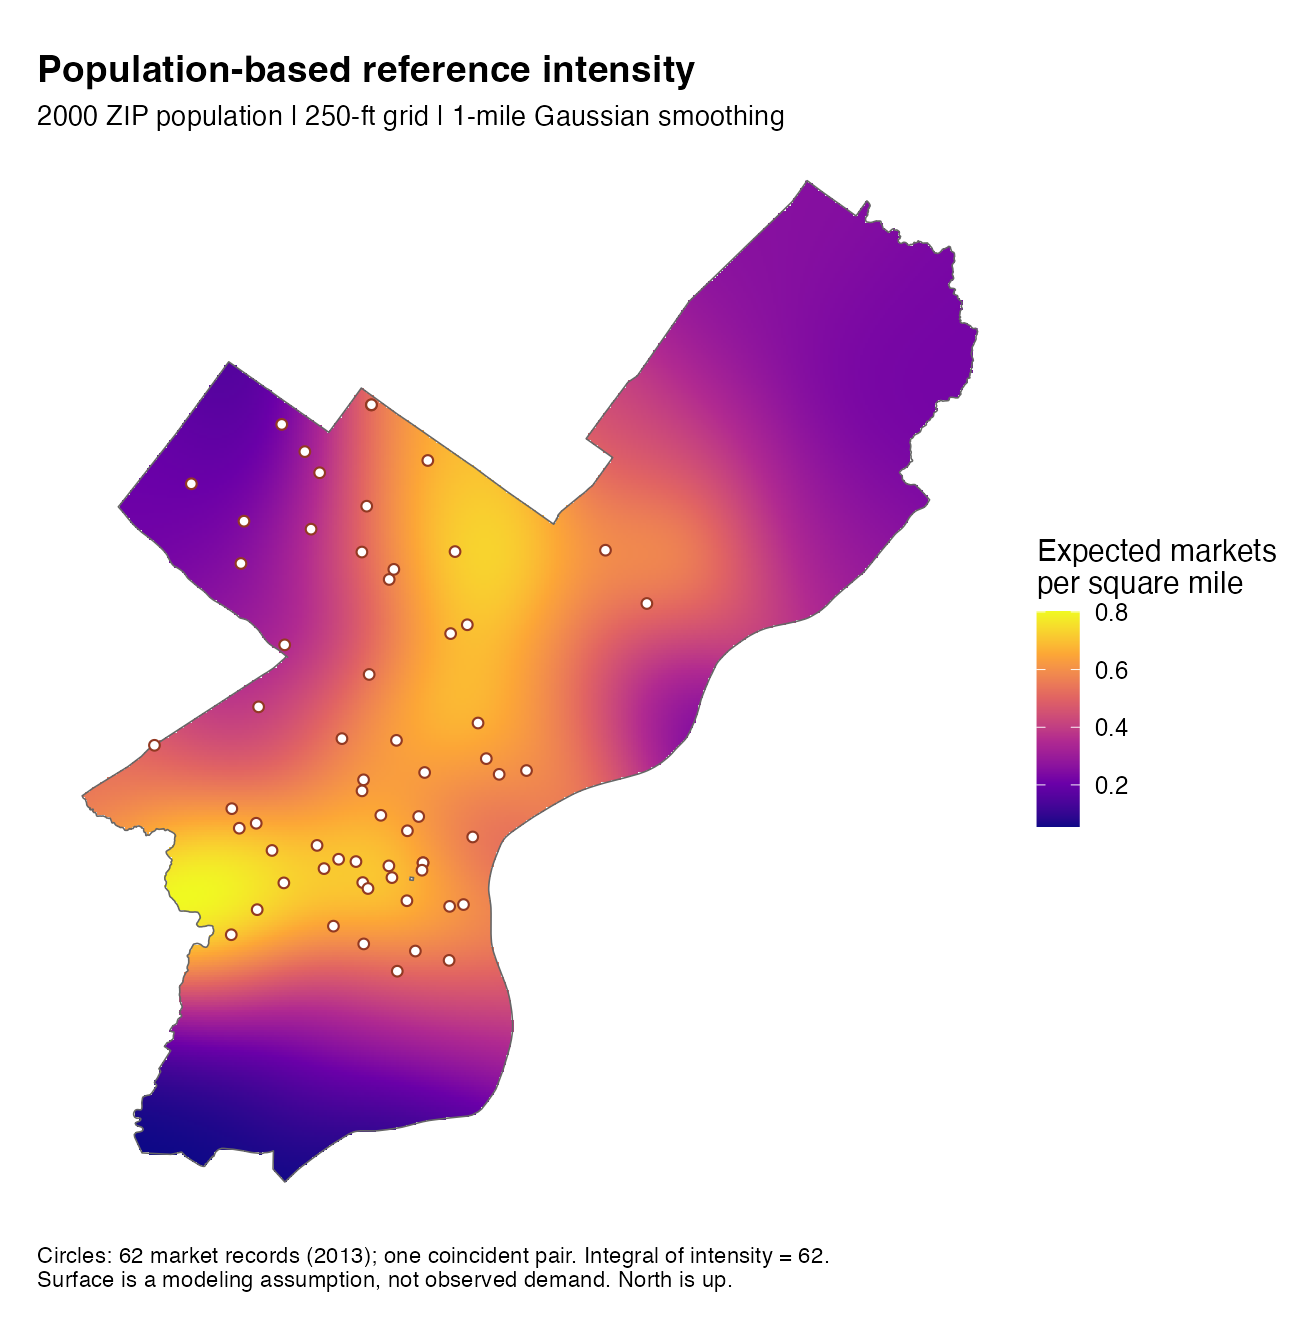
\includegraphics[width=0.75\linewidth]{../output/fig_07_lambda_intensity_map} 

}

\caption{Assumed population-proportional market intensity. The raster approximates ZIP population density; it does not reveal within-ZIP population or observed demand.}\label{fig:intensity-map}
\end{figure}

\section{D. Discussion}\label{d.-discussion}

\subsection{D.a. Agreement between nearest neighbor and K
results}\label{d.a.-agreement-between-nearest-neighbor-and-k-results}

Both methods reject \textbf{homogeneous CSR toward clustering}. Nearest
neighbor analysis finds a shorter average nearest-market distance than
the uniform reference; K finds excess cumulative pairs at every positive
reported band edge. Their agreement describes the observed arrangement
relative to a uniform citywide baseline. The population-based extension
addresses a different null and does not contradict that result.

\subsection{D.b. Visual expectations and method
limitations}\label{d.b.-visual-expectations-and-method-limitations}

The maps show many nearby markets in central and western neighborhoods
and large gaps in northeastern ZIPs, matching the homogeneous analyses.
However, the city includes very different residential and nonresidential
environments. NNA reduces the pattern to one distance per market; K
accumulates pairs over multiple scales and is sensitive to boundary
correction at large distances. Two records at Reading Terminal represent
one mapped location. ZIP smoothing, a one-mile bandwidth, a sample of 62
records, and the 2000/2013 time mismatch limit how specifically we can
interpret the adjusted result. Neither straight-line distance nor point
density measures prices, opening hours, transit access, or market
capacity.

\newpage

\begin{figure}

{\centering 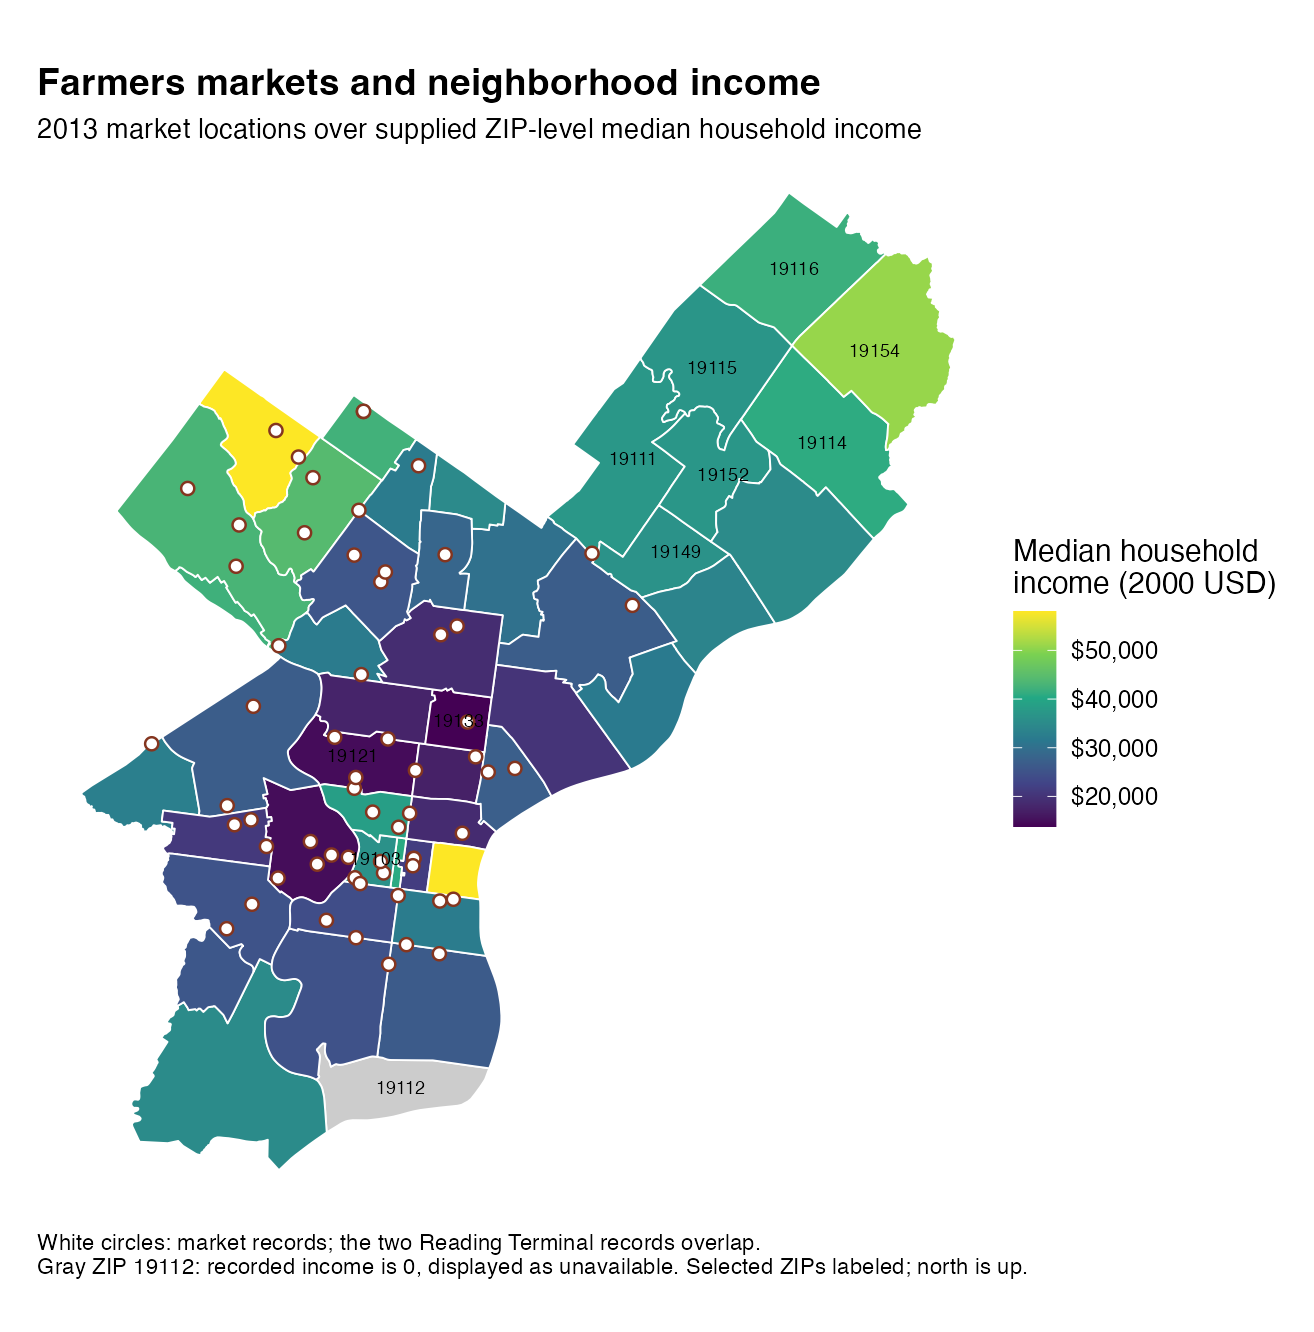
\includegraphics[width=0.75\linewidth]{../output/fig_09_income_map_markets} 

}

\caption{Required descriptive income map: 2013 farmers markets over 2000 median household income by ZIP. White circles denote markets; the coincident Reading Terminal pair overlaps.}\label{fig:income-map}
\end{figure}

\subsection{D.c. Median household income and market
presence}\label{d.c.-median-household-income-and-market-presence}

The map does \textbf{not} support a simple rule that lower-income ZIPs
always have fewer markets. Low-income ZIP 19104 (median household income
\$14,842) has five listed markets; 19121 (\$14,780) has two. ZIP 19133
(\$13,789) has one, whereas 19134 (\$20,067) has none. At the other end,
19118 (\$57,996) has two, but 19106 (\$58,018) has none. Several
northeastern ZIPs have moderate or higher incomes but no listed markets.
These contrasting examples support a mixed visual relationship, not an
income effect. No income association test was performed, as requested.
ZIP 19112's recorded income of zero is shown as unavailable rather than
interpreted as a zero-dollar household income.

\subsection{D.d. What can we conclude?}\label{d.d.-what-can-we-conclude}

The 2013 market records were clustered relative to a uniform
distribution within Philadelphia. We cannot infer that markets attract
one another, that population fully explains their locations, or that a
particular organization caused the pattern. Under our coarse
population-based Poisson reference, the observed adjusted K remains
within the envelope at all reported band edges. Nor does non-rejection
establish equitable access: a citywide curve can coexist with populated
ZIPs that contain no market.

\newpage

\subsection{D.e. Policy implications}\label{d.e.-policy-implications}

Planning should prioritize \textbf{populated areas with limited
fresh-food access}, rather than seek equal geographic spacing. The
northeastern ZIP examples are candidates for further investigation,
alongside low-income areas without markets such as 19134. Before
choosing sites, assess nearby grocery stores, transit and walking
routes, residents' needs, suitable operating space, and vendor demand.
Pilot markets or mobile markets could then be evaluated using attendance
and affordability measures.

Payment access also matters. In the supplied 2013 attributes, \textbf{49
of 62} records have \texttt{ACCEPT\_SNA\ =\ Yes}. The EBT field contains
40 \texttt{Yes}, 11 \texttt{Yes*}, and 11 \texttt{No}; the starred code
is preserved because its qualifier has not been verified. Policy
proposals could support payment equipment and nutrition-benefit
outreach, but these historical fields should be updated before
implementation. The results justify targeted investigation and community
engagement, not a claim that adding markets alone will resolve
food-access inequities.

\section{Data and references}\label{data-and-references}

\begin{itemize}
\tightlist
\item
  Course-supplied \textbf{HW 4 - Instructions.docx}, market and
  Philadelphia boundary shapefiles, and \textbf{Philadelphia\_ZipCodes}.
  Market vintage: 2013, attributed by the assignment to PASDA; ZIP
  population and median household income: 2000.
\item
  Group A/B scripts and outputs in
  \texttt{rowen37/MUSA-500-stats/assignment4}, retrieved at commit
  \texttt{a3e533b} (28 November 2026). Part C preserves their raw
  results and corrects interpretive wording in this integrated report.
\item
  \href{https://search.r-project.org/CRAN/refmans/spatstat.explore/html/Kest.html}{spatstat
  Kest},
  \href{https://search.r-project.org/CRAN/refmans/spatstat.explore/html/Lest.html}{Lest},
  \href{https://search.r-project.org/CRAN/refmans/spatstat.explore/html/Kinhom.html}{Kinhom},
  and
  \href{https://search.r-project.org/CRAN/refmans/spatstat.explore/html/envelope.html}{simulation
  envelopes}.
\item
  \href{https://pro.arcgis.com/en/pro-app/3.4/tool-reference/spatial-statistics/multi-distance-spatial-cluster-analysis.htm}{Esri:
  Multi-Distance Spatial Cluster Analysis}.
\end{itemize}

\textbf{Software disclosure:} Analysis and maps were produced in R. The
assignment's ArcGIS-specific Simulate Outer Boundary Values run and
graphical screenshot are not supplied; isotropic correction is a
documented substitute, not an equivalent implementation. The hospital
comparison is conceptual because the class slides were not included in
the repository. See \texttt{README.txt} for reproduction and integration
notes.

\end{document}
